% Technical report on the organisers' template (acmart, see kaggle_comp_report_fi_segm_2026.pdf).
% Text the template prints in BLACK is reproduced verbatim and must not change: the
% subtitle, the first sentence of the abstract, the first paragraph of the Introduction
% (with its footnote), the section titles, the Acknowledgment and references [1]-[2].
% Every result set in \Macro form comes from generated/numbers.tex, written by
% paper/make_figures.py from measured JSON. Do not type results by hand.
%
% Scope (author's instruction): only the submitted 0.41 solution, exp139 epoch 40, and the
% evaluation of that model (exp145). No other experiment appears here.
\documentclass[sigconf]{acmart}

\settopmatter{printacmref=false, printccs=false}
\setcopyright{none}
\copyrightyear{2026}
\acmYear{2026}
\acmDOI{}
\acmISBN{}
% acmart prints "short name, date, venue". The venue is empty here, so the date ends with
% \@gobble to swallow the separator comma, as in the organisers' sample footer.
\makeatletter
\acmConference[Kaggle Competition]{Solar Filament Segmentation Challenge 2026}{kaggle.com/competitions/filament-segmentation-2026\@gobble}{}
\makeatother

\usepackage{placeins}
\usepackage{tikz}
\usetikzlibrary{positioning,arrows.meta,fit,calc}
% Generated by paper/make_figures.py from measured JSON. Do not edit by hand.
\newcommand{\HostPQ}{0.4705}
\newcommand{\OurPQ}{0.4705}
\newcommand{\NumTP}{881}
\newcommand{\NumFP}{361}
\newcommand{\NumFN}{444}
\newcommand{\ValSQ}{0.685}
\newcommand{\ValRQ}{0.686}
\newcommand{\MeanIoUOverlap}{0.605}
\newcommand{\MeanDiceOverlap}{0.734}
\newcommand{\ValPhotos}{106}
\newcommand{\ValRecords}{180}
\newcommand{\ValGT}{1325}
\newcommand{\ValPred}{756}
\newcommand{\GTMissedPct}{18.5}
\newcommand{\GTOneOnePct}{78.7}
\newcommand{\GTSplitPct}{2.8}
\newcommand{\PredUnmatchedPct}{13.3}
\newcommand{\PredOneOnePct}{83.5}
\newcommand{\PredMergePct}{3.2}
\newcommand{\HumanPQ}{0.347}
\newcommand{\HumanPQAll}{0.340}
\newcommand{\HumanPairs}{1196}
\newcommand{\HumanValPairs}{202}
\newcommand{\HumanSQ}{0.636}
\newcommand{\HumanRQ}{0.546}
\newcommand{\SecondsPerPhoto}{2.49}
\newcommand{\InferenceGPU}{T4}
\newcommand{\TestMinutes}{7}
\newcommand{\PeakGiB}{2.7}
\newcommand{\LoadSeconds}{1.4}
\newcommand{\EpochFortyPQ}{0.4680}
\newcommand{\EpochFiftyPQ}{0.4636}
\newcommand{\BestEpoch}{40}
\newcommand{\RecallSmall}{0.45}
\newcommand{\RecallLarge}{0.75}
\newcommand{\PrecisionSmall}{0.55}
\newcommand{\PrecisionLarge}{0.82}
\newcommand{\SmallArea}{471}
\newcommand{\LargeArea}{3183}
\newcommand{\QualPQ}{0.478}
\newcommand{\QualMedian}{0.479}
\newcommand{\QualCandidates}{34}
\newcommand{\Submissions}{31}
\newcommand{\FirstPublic}{0.26}
\newcommand{\BestPublic}{0.41}
\newcommand{\FloatFortyPQ}{0.4705}
\newcommand{\FloatFiftyPQ}{0.4621}
\newcommand{\SoupPQ}{0.4688}
\newcommand{\FusionPQ}{0.4700}
\newcommand{\FusionExtraTP}{60}
\newcommand{\FusionExtraFP}{125}
\newcommand{\FailMissArea}{644}
\newcommand{\FailFPArea}{813}
\newcommand{\FailSplitArea}{14568}
\newcommand{\PQLow}{0.450}
\newcommand{\PQHigh}{0.491}
\newcommand{\SQLow}{0.680}
\newcommand{\SQHigh}{0.691}
\newcommand{\RQLow}{0.657}
\newcommand{\RQHigh}{0.715}
\newcommand{\HumanPQLow}{0.314}
\newcommand{\HumanPQHigh}{0.383}
\newcommand{\HumanPhotos}{47}
\newcommand{\RecallSmallLow}{0.39}
\newcommand{\RecallSmallHigh}{0.52}
\newcommand{\RecallLargeLow}{0.69}
\newcommand{\RecallLargeHigh}{0.80}
\newcommand{\PerBin}{221}
\newcommand{\AllPhotos}{707}
\newcommand{\AllRecords}{1154}
\newcommand{\AllFilaments}{8199}
\newcommand{\TrainPhotos}{601}
\newcommand{\TrainRecords}{974}
\newcommand{\TrainGT}{6874}


% Reference palette (dataviz skill, light mode). Text stays in ink colours.
\definecolor{vizblue}{HTML}{2A78D6}
\definecolor{vizorange}{HTML}{EB6834}
\definecolor{vizaqua}{HTML}{1BAF7A}
\definecolor{vizyellow}{HTML}{EDA100}
\definecolor{vizviolet}{HTML}{4A3AA7}
\definecolor{inkprimary}{HTML}{0B0B0B}
\definecolor{inksecondary}{HTML}{52514E}
\definecolor{inkmuted}{HTML}{898781}

\begin{document}

\title{Native-Resolution Mask2Former for Solar Filament Instance Segmentation}
\subtitle{A Solution to the Solar Filament Segmentation Challenge 2026}

% TODO(author): replace the institution, city, country and e-mail with your own.
\author{Ismail Kasozi}
\affiliation{%
  \institution{Your Institution}
  \city{City}
  \country{Country}}
\email{first.author@example.com}

\begin{abstract}
This report describes our solution to the Solar Filament Segmentation Challenge 2026, a
Kaggle competition on automatic segmentation of solar filaments in GONG H-$\alpha$
observations. Our solution is a single Mask2Former instance-segmentation network with a
Swin-S backbone that trains and predicts at the native $2048\times2048$ resolution.
Training mixes filament-centred crops with whole frames under exact dihedral
augmentation, and a fixed post-processing rule turns the per-query masks into disjoint
instances. On a validation split made by photograph and scored with the organisers'
self-evaluation notebook, the model reaches a Panoptic Quality (PQ) of \HostPQ{}
(95\% bootstrap interval \PQLow{}--\PQHigh{}). It scores \BestPublic{} on the public
leaderboard, with one forward pass of \SecondsPerPhoto{}\,s per photograph on a T4 GPU.
\end{abstract}

\maketitle

\section{Introduction}
This report goes over the details of our submitted solution to the Solar Filament
Segmentation Challenge 2026~\cite{challenge}. The challenge, launched on July 10, 2026,
is organized by the Earth-Space AI Research (ESAIR) Lab\footnote{www.esairlab.com/}.
This challenge utilizes the MAGFiLO dataset for evaluation of the segmentation
algorithms~\cite{magfilo}.

We treat the task as instance segmentation: each filament must be its own mask, and
every annotation record, one annotator's labels of one photograph, is scored against
the predictions for that photograph. Our submission is one model with one forward pass
per photograph: no test-time augmentation and no ensemble. Section~2 describes the
model, the data pipeline and the sampling strategy; Section~3 describes how we
evaluated it, including a run of the organisers' self-evaluation notebook on our
validation predictions.

\begin{figure*}[t]
\centering
\begin{tikzpicture}[
  font=\sffamily\scriptsize, >={Stealth[length=2mm]},
  box/.style={draw=#1, line width=0.8pt, fill=#1!9, rounded corners=2.5pt, minimum height=1.25cm,
              text width=1.82cm, align=center, inner sep=2.5pt, text=inksecondary,
              execute at begin node={\hyphenpenalty=10000}},
  head/.style={font=\sffamily\scriptsize\bfseries, text=inkprimary},
  flow/.style={->, line width=0.8pt, draw=inksecondary},
  lane/.style={font=\sffamily\scriptsize\bfseries, text=inkmuted, anchor=west}]
  % ---- training lane ----
  \node[lane] at (-1.05, 1.15) {TRAINING};
  \node[box=inkmuted] (data) at (0.4,0) {{\color{inkprimary}\textbf{MAGFiLO train file}}\\ \AllPhotos{} photographs\\ \AllRecords{} records};
  \node[box=inkmuted, right=0.27cm of data] (split) {{\color{inkprimary}\textbf{Photograph split}}\\ seed 2026\\ train \TrainPhotos{} / val \ValPhotos{}};
  \node[box=vizaqua, right=0.27cm of split] (samp) {{\color{inkprimary}\textbf{Sampling}}\\ 8 crops $1024^2$ on filaments, or 2 whole frames (25\%)};
  \node[box=vizaqua, right=0.27cm of samp] (aug) {{\color{inkprimary}\textbf{Augmentation}}\\ D4 flips \& turns;\\ gamma, gain};
  \node[box=vizviolet, right=0.27cm of aug] (fit) {{\color{inkprimary}\textbf{Set-prediction loss}}\\ Hungarian matching; CE, BCE, Dice};
  \node[box=vizviolet, right=0.27cm of fit] (opt) {{\color{inkprimary}\textbf{AdamW, 50 epochs}}\\ cosine decay,\\ bf16, batch 8};
  \node[box=inkmuted, right=0.27cm of opt] (pick) {{\color{inkprimary}\textbf{Checkpoint}}\\ epoch 40, best validation PQ};
  \foreach \a/\b in {data/split, split/samp, samp/aug, aug/fit, fit/opt, opt/pick} \draw[flow] (\a) -- (\b);
  % ---- inference lane ----
  \node[lane] at (-1.05, -1.6) {INFERENCE};
  \node (img) at (0.4,-2.85) {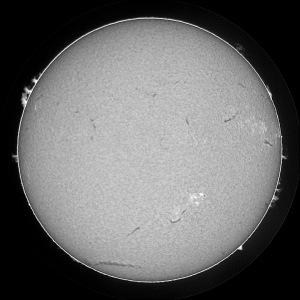
\includegraphics[width=1.25cm]{figures/thumb_input.png}};
  \node[font=\sffamily\scriptsize, text=inksecondary, below=-1pt of img, align=center] {H$\alpha$, $2048^2$};
  \node[box=inkmuted, right=0.27cm of img] (norm) {{\color{inkprimary}\textbf{Pre-processing}}\\ grey to 3 channels, ImageNet norm; no resizing};
  \node[box=vizblue, right=0.27cm of norm] (bb) {{\color{inkprimary}\textbf{Swin-S backbone}}\\ strides 4--32};
  \node[box=vizaqua, right=0.27cm of bb] (pd) {{\color{inkprimary}\textbf{Pixel decoder}}\\ multi-scale deformable attention};
  \node[box=vizviolet, right=0.27cm of pd] (td) {{\color{inkprimary}\textbf{Transformer decoder}}\\ 100 queries, masked attention};
  \node[box=vizorange, right=0.27cm of td] (hd) {{\color{inkprimary}\textbf{Query outputs}}\\ class probability, mask at stride 4};
  \node[box=vizyellow, right=0.27cm of hd] (pp) {{\color{inkprimary}\textbf{Post-processing}}\\ score $\geq 0.85$, paint by score, area $\geq 100$\,px};
  \node[right=0.3cm of pp] (out) {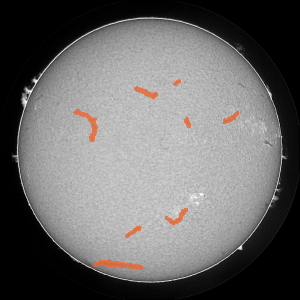
\includegraphics[width=1.25cm]{figures/thumb_output.png}};
  \node[font=\sffamily\scriptsize, text=inksecondary, below=-1pt of out, align=center] {RLE rows};
  \foreach \a/\b in {img/norm, norm/bb, bb/pd, pd/td, td/hd, hd/pp, pp/out} \draw[flow] (\a) -- (\b);
  \draw[->, line width=0.7pt, draw=inkmuted, dashed] (pick.south) -- ++(0,-0.55) -| node[pos=0.25, above, font=\sffamily\scriptsize, text=inkmuted] {trained weights} (bb.north);
\end{tikzpicture}
\caption{The end-to-end pipeline. Top: training, from the annotation file to the
selected checkpoint. Bottom: inference, one forward pass per test photograph at native
resolution in float32. Masks leave the network at stride 4 ($512\times512$ per frame)
and are upsampled to $2048\times2048$ before post-processing.}
\label{fig:pipeline}
\end{figure*}

\section{Methodology}
\subsection{Segmentation algorithm}
We use Mask2Former~\cite{mask2former}, an existing universal segmentation architecture,
in its instance-segmentation form. A backbone, here Swin-S~\cite{swin}, extracts
features at strides 4, 8, 16 and 32. A pixel decoder with multi-scale deformable
attention~\cite{deformabledetr} fuses them into per-pixel embeddings
$\mathbf{E}\in\mathbb{R}^{C\times H/4\times W/4}$. A Transformer decoder refines
$N=100$ learned queries; its cross-attention is \emph{masked}, so each query attends only
to the pixels its current mask covers. Each refined query $\mathbf{q}_i$ yields a class
distribution over \{filament, no object\} and a mask
\begin{equation}
\hat{\mathbf{m}}_i=\sigma\!\left(\mathbf{q}_i^{\top}\mathbf{E}\right)\in[0,1]^{H/4\times W/4}.
\end{equation}
Training matches queries to ground-truth filaments one-to-one with the Hungarian
algorithm~\cite{kuhn} and minimises
\begin{equation}
\mathcal{L}=\lambda_{\mathrm{cls}}\mathcal{L}_{\mathrm{CE}}
+\lambda_{\mathrm{mask}}\mathcal{L}_{\mathrm{BCE}}
+\lambda_{\mathrm{dice}}\mathcal{L}_{\mathrm{Dice}}
\end{equation}
with $(\lambda_{\mathrm{cls}},\lambda_{\mathrm{mask}},\lambda_{\mathrm{dice}})=(2,5,5)$,
the mask terms evaluated on sampled points and the no-object class weighted by 0.1, all
as in~\cite{mask2former}. We initialise from the COCO instance
model~\cite{coco}, replace the class head by one foreground class and train with
stochastic depth 0.3 (68.7\,M parameters in total).

\subsection{Data pipeline}
\textbf{Pre-processing.} Photographs stay grey and at $2048\times2048$; the channel is
repeated three times and normalised with ImageNet statistics. We never resize. The
reason is the mask resolution: Mask2Former predicts masks at a quarter of its input.
An ideal mask head on the stride-4 grid of a native input can reach a mean IoU of 0.914
with the annotated masks, but only 0.771 on the stride-8 grid that a $1024\times1024$
input would give (measured by downsampling the ground truth to each grid and back).
Ground-truth polygons are rasterised at native resolution with pycocotools, the
scorer's own convention.

\textbf{Post-processing.} The network outputs 100 candidates per photograph. The mask
logits are bilinearly upsampled to $2048\times2048$ and thresholded at probability 0.5.
Each candidate is scored as the product of its filament probability and its mean mask
probability inside the mask. Candidates with a score of at least 0.85 are painted in
descending score order; each keeps only the pixels that no higher-scoring candidate has
claimed, and it is dropped if fewer than 100 pixels remain. The instances are therefore
disjoint, as the scorer requires, and are written as RLE rows. The threshold and the
minimum area were chosen once, by a sweep on validation over 19 thresholds (0.05 to
0.95), two minimum areas (100 and 300 pixels) and optional one-pixel erosion.

\subsection{Sampling strategy and splits}
The training file holds \AllRecords{} annotation records of \AllPhotos{} distinct
photographs (\AllFilaments{} filaments); 296 photographs were annotated independently
by two or three people. If two records of one photograph sat on opposite sides of a
split, the model would be validated on a picture it had trained on, so we split by
photograph with a fixed seed (2026): \TrainPhotos{} photographs (\TrainRecords{}
records, \TrainGT{} filaments) for training and \ValPhotos{} photographs
(\ValRecords{} records, \ValGT{} filaments) for validation. The 180 test photographs
are held by the organisers. Every annotation record is a separate training sample,
because the metric scores each record against one annotator.

Each optimiser step holds either eight $1024\times1024$ crops or two whole frames, so
both kinds carry the same number of pixels; whole frames make up 25\% of the steps.
A crop is centred on a randomly chosen filament of its record, with jitter; 99\% of
training filaments are shorter than 516 pixels, so a crop almost always holds its
filament whole. Whole frames show the model the full disk and the off-disk background
at the scale it meets at inference. Augmentation applies the dihedral group D4 (flips
and $90^{\circ}$ turns, exact on the pixel grid), a gamma drawn log-uniformly from
$[0.8,1.25]$ and a gain from $[0.85,1.15]$.

\subsection{Training}
We train with AdamW~\cite{adamw}: learning rate $10^{-4}$, weight decay 0.05 (none on
norms and biases), a $0.1\times$ learning-rate multiplier on the backbone, gradient
clipping at 0.01, 500 warm-up steps and cosine decay. We train for 50 epochs
(12,150 steps) in bf16 on one H100 NVL GPU, at 0.47\,s per step (1.6 hours) and
39.4\,GiB peak memory. Every five epochs the run scores the validation split. We deploy
the checkpoint of epoch~40, the best of these scores (Section~\ref{sec:eval}). To make
training affordable we replaced the pure-PyTorch deformable attention by a compiled
CUDA kernel, batched the loss computation and moved photometric augmentation to the
GPU; each change was accepted only after a numerical test against the original code.

\begin{figure}[t]
\centering
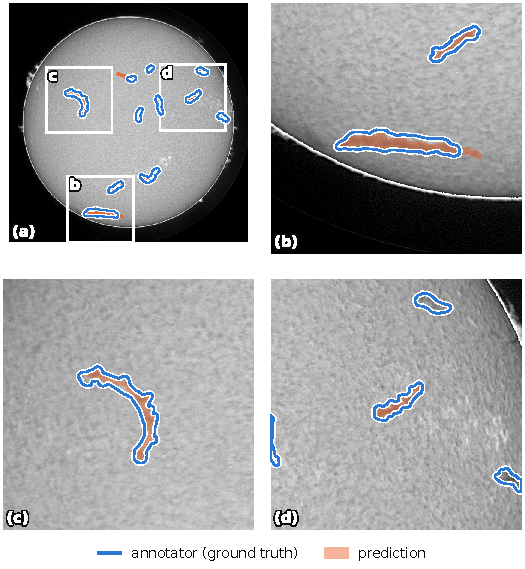
\includegraphics[width=\columnwidth]{figures/fig_qualitative.pdf}
\caption{Segmentations on the validation photograph whose PQ (\QualPQ{}) is closest to
the median of the \QualCandidates{} single-annotator validation photographs with at
least eight filaments (median \QualMedian{}); it is not a best case. (a) Full disk.
(b)--(d) Native-resolution zooms on the three largest annotated filaments. Blue: the
annotation, outlined 6\,px (16\,px on the disk) outside the mask so that the outline
never covers it. Orange: our prediction. Display contrast is stretched.}
\label{fig:qual}
\end{figure}

\section{Evaluation}\label{sec:eval}
\begin{figure*}[t]
\centering
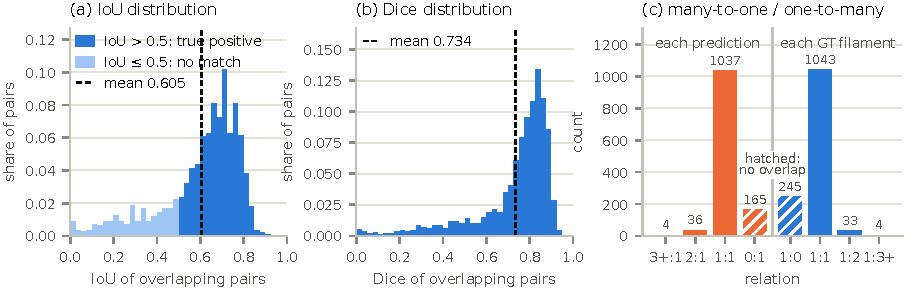
\includegraphics[width=\textwidth]{figures/fig_host_metrics.pdf}
\caption{The self-evaluation notebook's measures on our validation predictions.
(a) IoU of every overlapping (ground truth, prediction) pair; the darker bars pass the
0.5 threshold and count as true positives. (b) Dice of the same pairs.
(c) Predictions touching each ground-truth filament (right) and ground-truth filaments
touching each prediction (left); hatched bars have no overlap at all.}
\label{fig:host}
\end{figure*}

\begin{figure}[t]
\centering
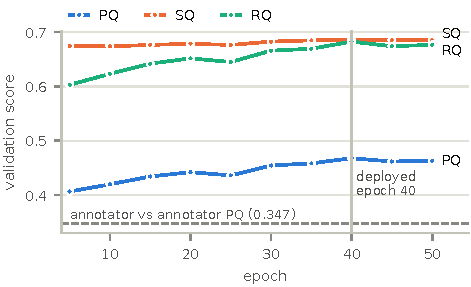
\includegraphics[width=\columnwidth]{figures/fig_curve.pdf}
\caption{Validation PQ, SQ and RQ by epoch from the evaluation inside training (bf16
inference) at the deployed rule. Dashed: annotator-versus-annotator PQ.}
\label{fig:curve}
\end{figure}

\begin{figure}[t]
\centering
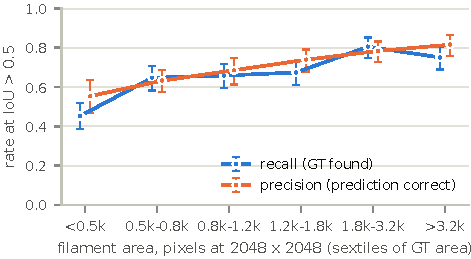
\includegraphics[width=\columnwidth]{figures/fig_size.pdf}
\caption{Recall (ground-truth filaments found at IoU $>0.5$) and precision (predictions
that match) by filament area, in sextiles of ground-truth area (\PerBin{} filaments per
bin). Bars: Wilson 95\% intervals.}
\label{fig:size}
\end{figure}

\begin{figure}[t]
\centering
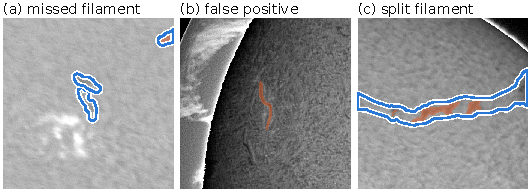
\includegraphics[width=\columnwidth]{figures/fig_failures.pdf}
\caption{One example of each error, chosen by a fixed rule over single-annotator
validation records: (a) the median-area filament that no prediction touches; (b) the
median-area prediction that touches no filament; (c) the largest filament touched by two
or more predictions. Colours as in Figure~\ref{fig:qual}.}
\label{fig:failures}
\end{figure}

\subsection{Evaluation strategy}
A (ground truth, prediction) pair with IoU above 0.5 is a true positive; unmatched
predictions are false positives and unmatched ground-truth filaments false negatives;
the counts are pooled over all records and
$\mathrm{PQ}=\sum_{\mathrm{TP}}\mathrm{IoU}/(|\mathrm{TP}|+\tfrac12|\mathrm{FP}|+\tfrac12|\mathrm{FN}|)
=\mathrm{SQ}\times\mathrm{RQ}$~\cite{pq}. We ran the organisers' self-evaluation notebook
verbatim on our validation predictions. It returns PQ 0.4705249989 and our own
evaluator 0.4705249990, with identical counts, so all validation numbers here measure
the leaderboard's quantity. Uncertainty comes from a bootstrap~\cite{bootstrap}
that resamples the \ValPhotos{} validation photographs 10,000 times; a photograph's
records share one set of predictions, so they are resampled together. Rates carry Wilson
95\% intervals~\cite{wilson}. To read the scores we also scored each annotator
against every other annotator of the same validation photograph under the same rule.

\begin{table}[t]
\caption{Validation results (106 photographs, 180 records, host notebook). Brackets:
95\% bootstrap intervals over photographs.}
\label{tab:results}
\small
\setlength{\tabcolsep}{3pt}
\newcommand{\ci}[2]{{\scriptsize[#1, #2]}}
\begin{tabular}{@{}lccc@{}}
\toprule
 & PQ & SQ & RQ \\
\midrule
Our model, epoch 40 & \HostPQ{} & \ValSQ{} & \ValRQ{} \\
 & \ci{\PQLow}{\PQHigh} & \ci{\SQLow}{\SQHigh} & \ci{\RQLow}{\RQHigh} \\
\quad TP / FP / FN & \multicolumn{3}{c}{\NumTP{} / \NumFP{} / \NumFN{}} \\
Annotator vs annotator & \HumanPQ{} & \HumanSQ{} & \HumanRQ{} \\
 & \ci{\HumanPQLow}{\HumanPQHigh} & & \\
\midrule
Public leaderboard (test) & \BestPublic{} & -- & -- \\
\bottomrule
\end{tabular}
\end{table}

\subsection{Results}
Table~\ref{tab:results} summarises the validation scores. Our model agrees with a held-out
annotator more closely than two annotators agree with each other, and the two
intervals do not overlap. A model trained on many annotators learns their average,
which can sit closer to each of them than they sit to each other, so this is a
reference for label variability rather than a claim of super-human skill. The
public leaderboard shows \BestPublic{}. It is scored on a different set of photographs
and annotators and shown to two decimals, so it is not directly comparable with the
validation interval.


Figure~\ref{fig:host} shows the distributions the notebook reports. Overlapping pairs
have a mean IoU of \MeanIoUOverlap{} and a mean Dice of \MeanDiceOverlap{}. Of the
ground-truth filaments, \GTOneOnePct{}\% touch exactly one prediction,
\GTSplitPct{}\% touch two or more (fragmentation) and \GTMissedPct{}\% touch none. Of the
predictions, \PredOneOnePct{}\% touch exactly one filament, \PredMergePct{}\% touch two
or more (merging) and \PredUnmatchedPct{}\% touch none.


Figure~\ref{fig:curve} shows the scores during training. PQ peaks at epoch
\BestEpoch{} and then drifts down while SQ stays flat, so the late decline comes from
recognition, not from mask quality. Because epoch~40 was selected on the same
validation split, its validation score is slightly optimistic.



\subsection{Strengths, weaknesses and improvements}
\textbf{Strengths.} Filaments are rarely split or merged (\GTSplitPct{}\% and
\PredMergePct{}\%): each query proposes one whole filament, and painting by score
keeps the instances disjoint without a separate merging step. Masks are accurate once a
filament is found (SQ \ValSQ{}). The whole test set runs in about \TestMinutes{} minutes
on one T4 GPU (\SecondsPerPhoto{}\,s per photograph, \PeakGiB{}\,GiB of memory).

\textbf{Weaknesses.} The model misses filaments far more often than it invents them:
\NumFN{} false negatives against \NumFP{} false positives. Figure~\ref{fig:size} shows
where: recall is \RecallSmall{} [\RecallSmallLow{}, \RecallSmallHigh{}] for the
smallest sixth of filaments (under \SmallArea{} pixels) against \RecallLarge{}
[\RecallLargeLow{}, \RecallLargeHigh{}] for the largest. Figure~\ref{fig:failures}(a)
shows a typical miss, a small faint structure (\FailMissArea{} pixels). Some false
positives are dark structures that the annotator did not mark
(Figure~\ref{fig:failures}(b)), and long filaments are occasionally covered by several
predictions (Figure~\ref{fig:failures}(c)).

\textbf{Improvements.} Three changes address these weaknesses directly. First, train
on all \AllRecords{} records once the recipe is fixed, adding 18\% more annotations.
Second, recover small filaments with a verification stage that examines candidates
scoring below the 0.85 threshold. Third, use the 296 multiply-annotated photographs to
build consensus targets, which should reduce the noise in the training signal.

\FloatBarrier
\section{Acknowledgment}
The organization of the Filament Segmentation Challenge 2026 is partially supported by
the U.S. National Science Foundation (NSF) under Grant No. 2209912 and 2433781,
directorate for Computer and Information Science and Engineering (CSE), and Office of
Advanced Cyberinfrastructure (OAC), and Grant No. 2511630, AST Division Of Astronomical
Sciences and MPS Directorate for Mathematical and Physical Sciences.

The Filament Segmentation Challenge 2026 is sponsored by the U.S. National Science
Foundation (NSF) National Solar Observatory (NSO).

This work utilizes GONG data obtained by the NSO Integrated Synoptic Program, managed
by the National Solar Observatory, which is operated by the Association of Universities
for Research in Astronomy (AURA), Inc. under a cooperative agreement with the National
Science Foundation and with contribution from the National Oceanic and Atmospheric
Administration. The GONG network of instruments is hosted by the Big Bear Solar
Observatory, High Altitude Observatory, Learmonth Solar Observatory, Udaipur Solar
Observatory, Instituto de Astrofísica de Canarias, and Cerro Tololo Interamerican
Observatory.

\bibliographystyle{ACM-Reference-Format}
\bibliography{refs}

\end{document}
